So, the distance between the given planes is:
\begin{align}
   \frac{\abs{4 - 6}}{\sqrt{2^2+3^2+4^2}}   =   \frac{2}{\sqrt{29}}    
\end{align}
See Fig.        \ref{fig:parallel_planessolutions/line_plane/110/}

\begin{figure}[t]
    \centering
    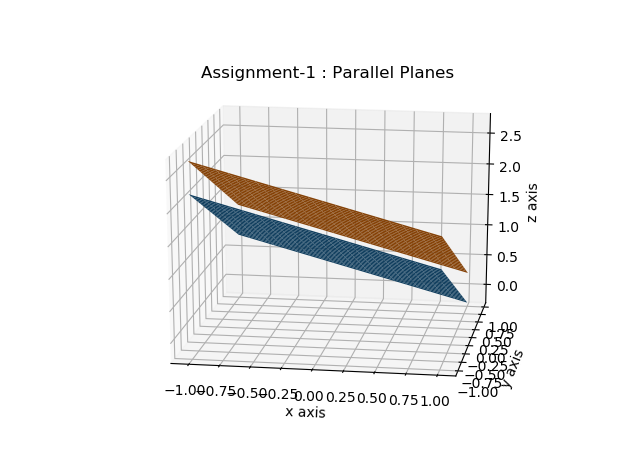
\includegraphics[width = \columnwidth]{./solutions/line_plane/110/parallel planes.png}
    \caption{Example of Two parallel planes}
    \label{fig:parallel_planessolutions/line_plane/110/}
\end{figure}

